\documentclass{beamer}
\usepackage{graphicx}
\usepackage{paralist}
\usepackage{outlines}

\title{Photo Correction Filters}
\author{Mendocino College - Digital Image Manipulation with Photoshop}
\titlegraphic{\vspace{-10mm}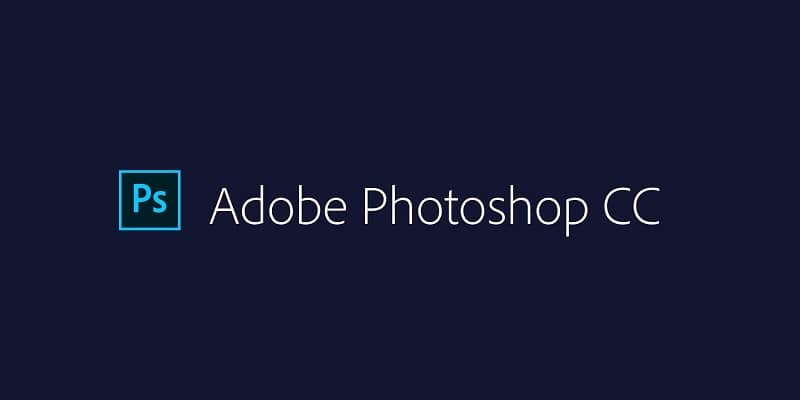
\includegraphics[width = .9\textwidth]{images/photoshop.jpg}} 
\date{\vspace{-5em}} 


\mode <presentation>
\usetheme{Warsaw}
\usecolortheme{default}

\setbeamerfont{footline}{size=\fontsize{5}{8}\selectfont}

\definecolor{darkred}{rgb}{20,0,0}
\definecolor{darkgreen}{RGB}{40,110,20}
\definecolor{darkpurple}{RGB}{30,0,30}
\definecolor{chardonnay}{RGB}{255, 255, 204}

\setbeamercolor*{palette primary}{fg=white, bg=darkgreen}


\begin{document}
	{
		\setbeamertemplate{footline}{} 
		\setbeamertemplate{headline}{} 
		\begin{frame}
			\vspace{-35pt}
			\maketitle
		\end{frame}
	}


		\section{}
			\subsection{Photo Corrections}		
			\begin{frame}
				\frametitle{Photo Corrections}
				\begin{outline}
					\1 Most of your basic photo corrections will be working with color corrections.
					\1 Now we will look into using filters to correct for specific issues
				\end{outline}
			\end{frame}
		
		\section{Camera Raw Filter}
\subsection{Filter}		
\begin{frame}
	\frametitle{Camera Raw Filter}
	\begin{outline}
		\1 Adobe Camera Raw Filter is a Photoshop plug-in for making color and tonal adjustments.
		\1 In its editing window, there is a large preview image and the adjustment tools are laid out in the order that you would normally use them. 
		\1 If you want to apply the same adjustment to multiple images, you can save the settings as a preset and apply as needed.  
		\1 $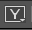
\includegraphics[width=0.05\textwidth]{images/camera raw - split.png}$ Switches between Before/After modes
	\end{outline}
\end{frame}

\subsection{Example}		
\begin{frame}
	\frametitle{Camera Raw Filter Example}
	\begin{center}
	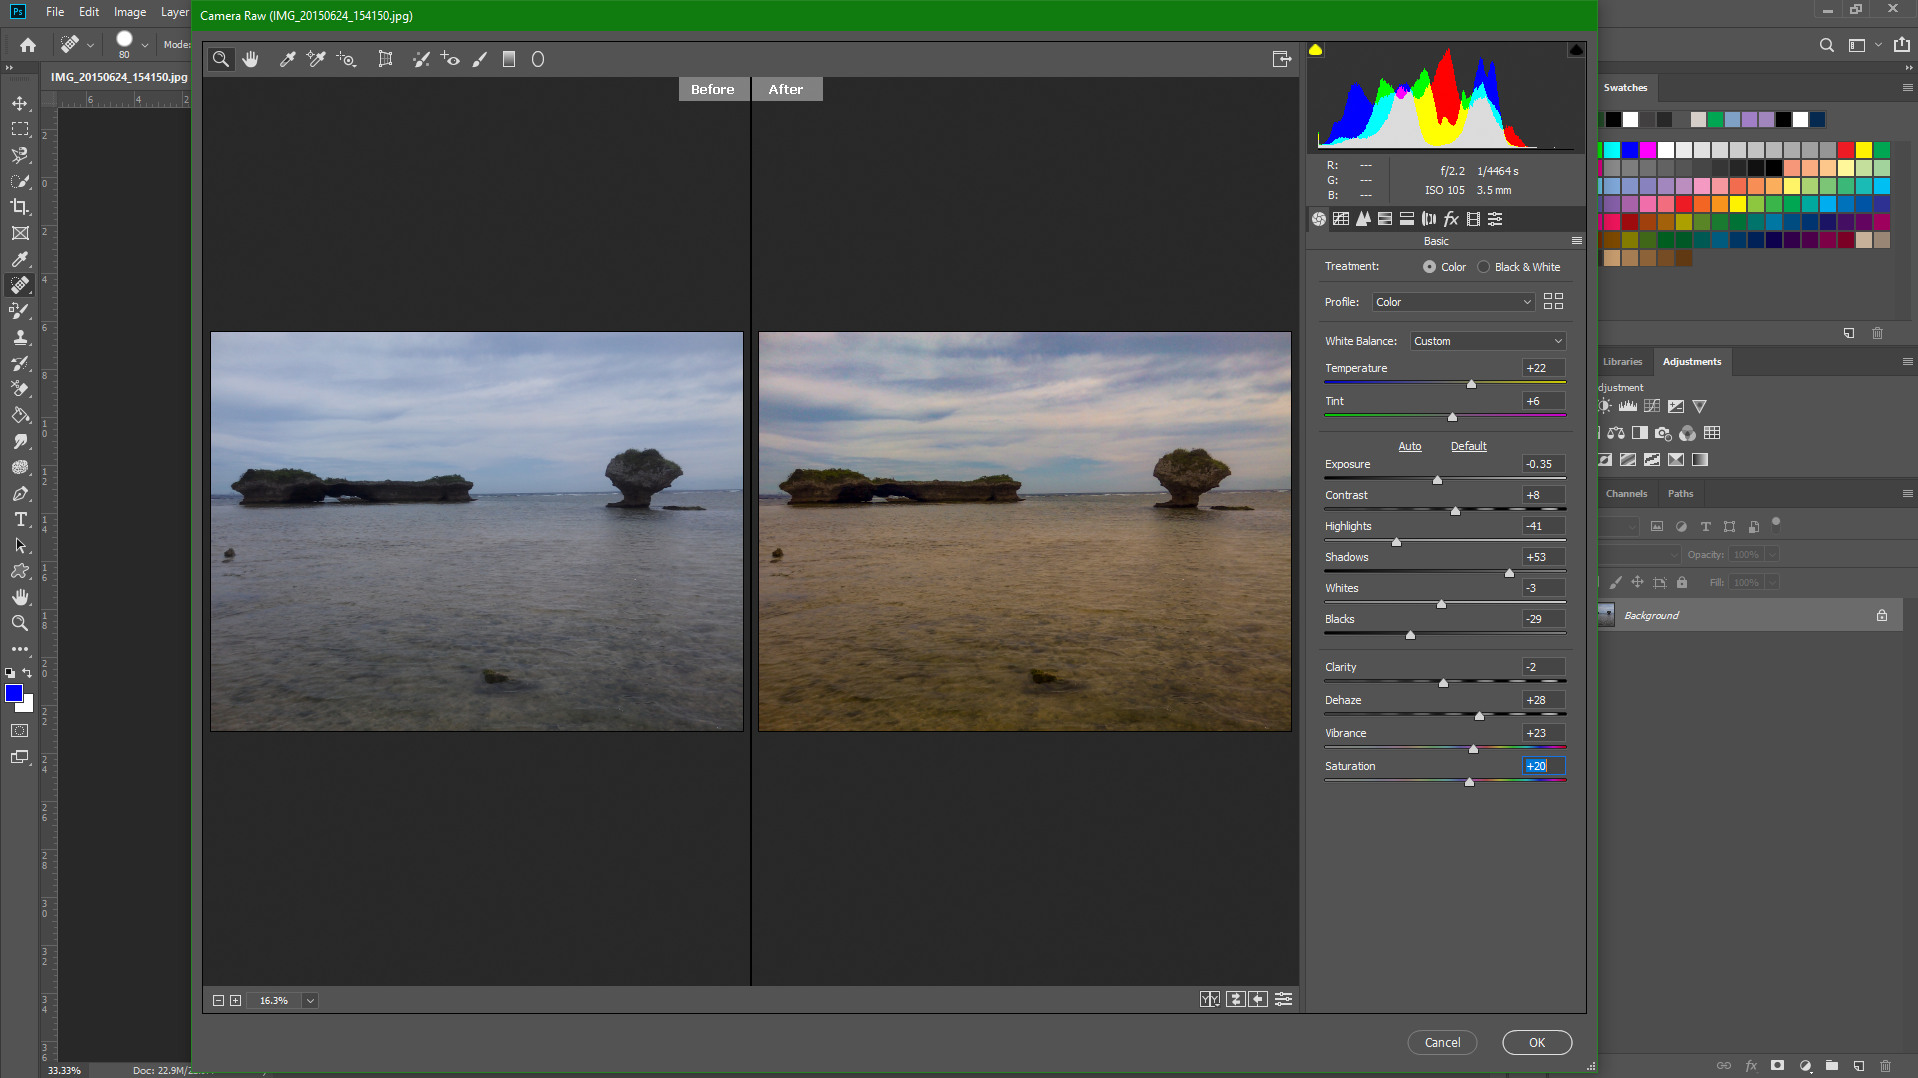
\includegraphics[width=1.10\textwidth]{images/Camera raw filter example.png}
	\end{center}
\end{frame}

\subsection{Options}		
\begin{frame}
	\frametitle{Camera Raw Options}
	\begin{outline}
		\1 Basic - All of your basic adjustment options, such as contrast/exposure/vibrance/etc
		\1 Tone Curve - Similar to Curves adjustment layer, but for the highlights/Lights/Darks/Shadows
		\1 Detail - Adjustment sliders for Sharpening and Noise
		\1 HSL Adjustments - Sliders to adjust Hue, Saturation, and Luminance.
		\1 Split Toning - Hue/Saturation sliders for Highlights and Shadows.
		\1 Lens Correction - Sliders to adjust Distortion, Defringe, Vignetting.
		\1 Effects - Sliders to adjust Grain and Post Crop Vignetting.
		\1 Calibration - Slider to adjust Shadows, Red Primary, Green Primary, Blue Primary.
		\1 Presets - Preset adjustments to easily apply to images.
	\end{outline}
\end{frame}

		\section{Adaptive Wide Angle Filter}
			\subsection{Filter}		
			\begin{frame}
				\frametitle{Adaptive Wide Angle filter}
				\begin{outline}
					\1 The Adaptive Wide Angle filter to correct lens distortions due to using wide angle lenses.
					\1 Straighten lines that appear curved in panoramas, or photos taken with fish-eye and wide angle lenses.
					\1 The filter detects the camera and lens model and uses the lens characteristics to straighten the images. 
					\1 You can add multiple constraints to indicate straight lines in different parts of the picture. 
					\2 Using this information, the Adaptive Wide Angle filter removes the distortions.
					\2 You can also use this filter on images that do not contain camera and lens information, though it's some extra work.
				\end{outline}
			\end{frame}
		
		\subsection{Example}		
		\begin{frame}
			\frametitle{Adaptive Wide Angle filter Example}
			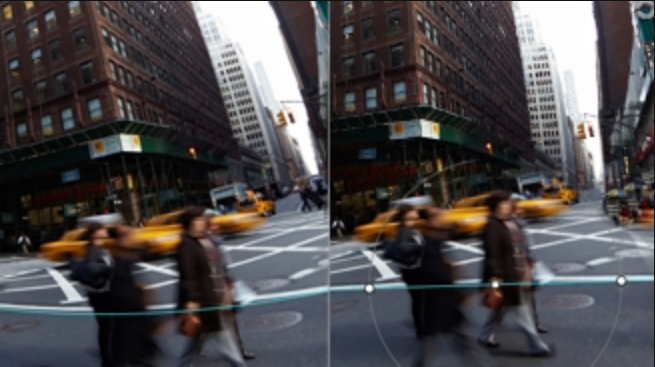
\includegraphics[width=1.0\textwidth]{images/Adaptive Wide Angle filter.png}
		\end{frame}
	
				\subsection{Options}		
	\begin{frame}
		\frametitle{Adaptive Wide Angle filter Options}
		\begin{outline}
			\1 Crop Factor - Specify a value to determine how the final image is cropped. Use this value in combination with Scale to compensate for any blank areas that are introduced while applying the filter. 
			\1 Correction Types:
			\2 Fisheye - Corrects extreme curvature caused by a fisheye lens.
			\2 Perspective - Corrects converging lines caused by angle of view and camera tilt.
			\2 Panorama - Corrects a Photomerge panorama.
			\2 Full Spherical - Corrects 360-degree panoramas. The panoramas must have a 2:1 aspect ratio.
			\2 Auto - Detects the appropriate correction automatically.
			\1 If you want to edit the filter settings later, convert the layer to a smart object. Select the layer and choose:  Layers $\rightarrow$ Smart Objects $\rightarrow$ Convert to Smart Object.
		\end{outline}
	\end{frame}

\begin{frame}
	\frametitle{Adaptive Wide Angle filter Options}
	\begin{outline}
		\1 If the image has lens data, these values are automatically detected, and some options are not displayed.
		\1 Focal Length - Specify the focal length of the lens. This value is automatically populated if the lens information is detected in the photograph.
		\1 Scale - Specify a value to scale the image. Use this value to minimize the blank areas that are introduced after applying the filter.
		\1 Focal Length - Specify the focal length of the lens. This value is automatically populated
		if the lens information is detected in the photograph.
		\1 Crop Factor - Specify a value to determine how the final image is cropped. Use this value
		in combination with Scale to compensate for any blank areas that are introduced while applying the filter.
		\1 As Shot - Enable this option to use the values as defined in the lens profile. This option is disabled if no lens information is found.
	\end{outline}
\end{frame}

				\subsection{Resources}		
\begin{frame}
	\frametitle{Additional Resource for using the Adaptive Wide Angle filter}
	\begin{outline}
		\1 Walk-through example using 11-steps to correct an image.
		\2 https://creativepro.com/how-to-use-the-adaptive-wide-angle-filter-in-photoshop/
		\1 Quick video walk-through how to use the filter.
		\2 https://www.youtube.com/watch?v=2qSEIHXkFsM
	\end{outline}
\end{frame}
			
		\section{Lens Correction Filter}
			\subsection{Distortions}		
			\begin{frame}
				\frametitle{Lens Distortions}
								\begin{outline}
					\1 Barrel distortion is a lens defect that causes straight lines to bow out toward the edges of the image.
					\1 Pincushion distortion is the opposite effect, where straight lines bend inward.
					\1 Vignetting is a defect that darkens the corners of an image due to light falloff around the perimeter of the lens. 
					\1 Chromatic aberration appears as a color fringe along the edges of objects, caused by the lens focusing on different colors of light in different planes.
					\1 Some lenses exhibit different defects at certain focal lengths, f‑stops, and focus distances. With the Lens Correction filter, you can specify the combination of settings used to make the image.
				\end{outline}
			\end{frame}
		
					\subsection{Filter}		
		\begin{frame}
			\frametitle{Lens Correction Filter}
			\begin{outline}
				\1 The Lens Correction filter fixes common lens flaws such as barrel and pincushion distortion, vignetting, and chromatic aberration. 
				\1 The filter works only with 8‑ and 16‑bit-per-channel images in RGB or Grayscale mode.
				\1 You can also use the filter to rotate an image or fix image perspective caused by vertical or horizontal camera tilt. 
				\1 The filter’s image grid makes these adjustments easier and more accurate than using the Transform command.
			\end{outline}
		\end{frame}
		
					\subsection{Example}		
		\begin{frame}
			\frametitle{Lens Correction Filter Example}
			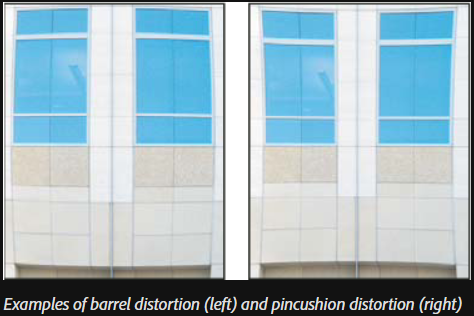
\includegraphics[width=1.0\textwidth]{images/Lens Correction Filter Example.png}
		\end{frame}
	
						\subsection{Options}		
	\begin{frame}
		\frametitle{Lens Correction Options}
		\begin{outline}
			\1 Correction - Select the problems you want to fix. If corrections undesirably extend or contract the image beyond original dimensions, select Auto Scale Image.
			\1 The Edge menu specifies how to handle blank areas that result from pincushion, rotation, or perspective corrections. You can fill blank areas with transparency or a color, or you can extend the edge pixels of the image.
			\1 Search Criteria - Filters the Lens Profiles list. 
			\2 By default, profiles based on image sensor size appear first. 
			\2 To list RAW profiles first, click the pop-up menu , and select Prefer RAW Profiles.
		\end{outline}
	\end{frame}

	\begin{frame}
	\frametitle{Lens Correction Options}
	\begin{outline}
		\1 Lens Profiles - 
		\2 By default, Photoshop displays only profiles that match the camera and lens used to create the image. (The camera model does not have to match perfectly.) 
		\2 Photoshop automatically selects a matching sub-profile for the selected lens based on focal length, f-stop and focus distance. 
		\2 To change the automatic selection, right-click the current lens profile, and select a different sub-profile.
		\1 Remove Distortion - 
		\2 Corrects lens barrel or pincushion distortion. 
		\2 Move the slider to straighten horizontal and vertical lines that bend either away from or toward the center of the image. 
		\2 Drag toward the center of the image to correct for barrel distortion and toward the edge of the image to correct for pincushion distortion. 
		\2 If any blank image edges result, adjust the Edge option on the Auto Correction tab.
	\end{outline}
\end{frame}

					\subsection{Resources}		
	\begin{frame}
		\frametitle{Additional Resource for using the Lens Correction filter}
		\begin{outline}
			\1 Adobe's guide for lens and noise correction.
			\2 https://helpx.adobe.com/photoshop/using/correcting-image-distortion-noise.html
			\1 Manual Lens Correction
			\2 https://expertphotography.com/photoshop-lens-correction/
		\end{outline}
	\end{frame}
	
	
		\section{Vanishing Point Filter}
			\subsection{Filter}		
				\begin{frame}
					\frametitle{Vanishing Point Filter}
					\begin{outline}
						\1 Vanishing Point simplifies perspective-correct editing in images that contain perspective planes
						\2 for example, the sides of a building, walls, floors, or any rectangular object.
						\1 You specify the planes in an image, and then apply edits such as painting, cloning, copying or pasting, and transforming. 
						\1 All your edits honor the perspective of the plane you’re working in. 
						\1 When you retouch, add, or remove content in an image, the results are more realistic because the edits are properly oriented and scaled to the perspective planes. 
						\1 After you finish working in Vanishing Point, you can continue editing the image in Photoshop.
					\end{outline}
				\end{frame}
			
			\subsection{Example}		
	\begin{frame}
		\frametitle{Vanishing Point Filter Example}
		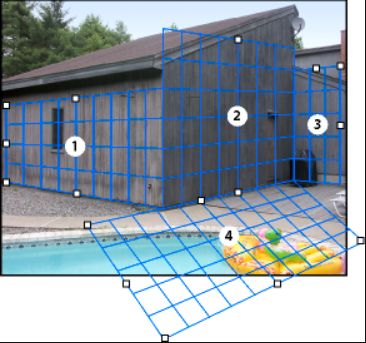
\includegraphics[width=0.9\textwidth]{images/vanishing point example.png}
	\end{frame}

			\subsection{Options}		
\begin{frame}
	\frametitle{Vanishing Point Filter Dialog Box}
	\begin{center}
	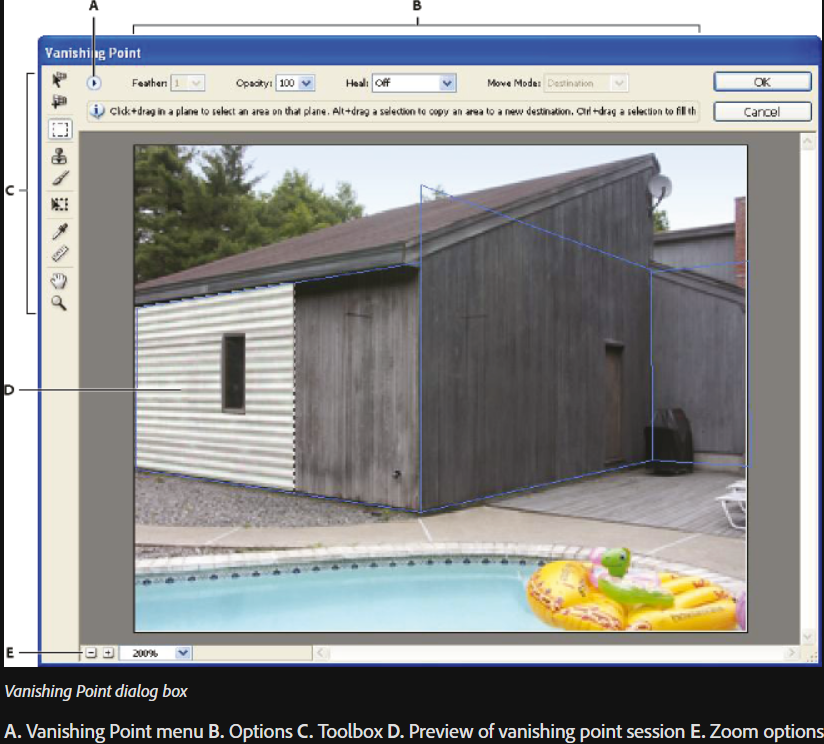
\includegraphics[width=0.75\textwidth]{images/vanishing point dialog box.png}
	\end{center}
\end{frame}

				\begin{frame}
	\frametitle{Vanishing Point Tools}
	\begin{outline}
		\1 Create Plane tool - Defines the four corner nodes of a plane, adjusts the size and shape of the plane, and tears off a new plane.
		\1 Edit Plane tool - Selects, edits, moves, and resizes planes.
		\1 Marquee tool - Makes square or rectangular selections, and also moves or clones selections.
		\1 Stamp tool - Paints with a sample of the image. Unlike the Clone Stamp tool, the Stamp tool in Vanishing Point can’t clone elements from another image. 
		\1 Measure tool - Measures distances and angles of an item in a plane. See also Measure in Vanishing Point
		\1 Transform tool - Scales, rotates, and moves a floating selection by moving the bounding box handles. Its similar to using the Free Transform command on a rectangle selection. 
		\1 Eyedropper tool - Selects a color for painting.
	\end{outline}
\end{frame}

				\subsection{Resources}		
\begin{frame}
	\frametitle{Additional Resource for using the Vanishing Point filter}
	\begin{outline}
		\1 Adobe's walkthrough for working with Vanishing Point
		\2 https://helpx.adobe.com/sg/photoshop/using/vanishing-point.html
	\end{outline}
\end{frame}



		\section{}
			\subsection{Destructive Edits}		
			\begin{frame}
				\frametitle{Destructive Edits}
				\begin{outline}
					\1 Applying some of these tools permanently alters the image information.
					\1 It is recommended to always work using nondestructive edits.
					\1 To edit your images nondestructively, always work on a duplicate layer. 
				\end{outline}
				\begin{center}
					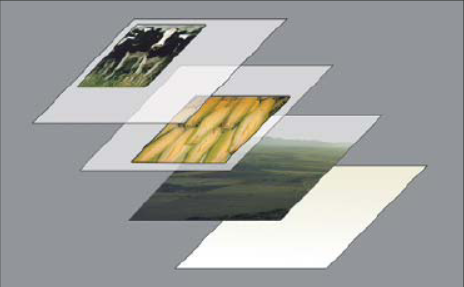
\includegraphics[width=0.7\textwidth]{images/layers example.png}
				\end{center}	
			\end{frame}
	
\end{document}